% Options for packages loaded elsewhere
% Options for packages loaded elsewhere
\PassOptionsToPackage{unicode}{hyperref}
\PassOptionsToPackage{hyphens}{url}
\PassOptionsToPackage{dvipsnames,svgnames,x11names}{xcolor}
%
\documentclass[
  article,
  nofooter,
  noheadings]{jss}
\usepackage{xcolor}
\usepackage{amsmath,amssymb}
\setcounter{secnumdepth}{-\maxdimen} % remove section numbering
\usepackage{iftex}
\ifPDFTeX
  \usepackage[T1]{fontenc}
  \usepackage[utf8]{inputenc}
  \usepackage{textcomp} % provide euro and other symbols
\else % if luatex or xetex
  \usepackage{unicode-math} % this also loads fontspec
  \defaultfontfeatures{Scale=MatchLowercase}
  \defaultfontfeatures[\rmfamily]{Ligatures=TeX,Scale=1}
\fi
\usepackage{lmodern}
\ifPDFTeX\else
  % xetex/luatex font selection
\fi
% Use upquote if available, for straight quotes in verbatim environments
\IfFileExists{upquote.sty}{\usepackage{upquote}}{}
\IfFileExists{microtype.sty}{% use microtype if available
  \usepackage[]{microtype}
  \UseMicrotypeSet[protrusion]{basicmath} % disable protrusion for tt fonts
}{}
\makeatletter
\@ifundefined{KOMAClassName}{% if non-KOMA class
  \IfFileExists{parskip.sty}{%
    \usepackage{parskip}
  }{% else
    \setlength{\parindent}{0pt}
    \setlength{\parskip}{6pt plus 2pt minus 1pt}}
}{% if KOMA class
  \KOMAoptions{parskip=half}}
\makeatother
% Make \paragraph and \subparagraph free-standing
\makeatletter
\ifx\paragraph\undefined\else
  \let\oldparagraph\paragraph
  \renewcommand{\paragraph}{
    \@ifstar
      \xxxParagraphStar
      \xxxParagraphNoStar
  }
  \newcommand{\xxxParagraphStar}[1]{\oldparagraph*{#1}\mbox{}}
  \newcommand{\xxxParagraphNoStar}[1]{\oldparagraph{#1}\mbox{}}
\fi
\ifx\subparagraph\undefined\else
  \let\oldsubparagraph\subparagraph
  \renewcommand{\subparagraph}{
    \@ifstar
      \xxxSubParagraphStar
      \xxxSubParagraphNoStar
  }
  \newcommand{\xxxSubParagraphStar}[1]{\oldsubparagraph*{#1}\mbox{}}
  \newcommand{\xxxSubParagraphNoStar}[1]{\oldsubparagraph{#1}\mbox{}}
\fi
\makeatother


\usepackage{longtable,booktabs,array}
\usepackage{calc} % for calculating minipage widths
% Correct order of tables after \paragraph or \subparagraph
\usepackage{etoolbox}
\makeatletter
\patchcmd\longtable{\par}{\if@noskipsec\mbox{}\fi\par}{}{}
\makeatother
% Allow footnotes in longtable head/foot
\IfFileExists{footnotehyper.sty}{\usepackage{footnotehyper}}{\usepackage{footnote}}
\makesavenoteenv{longtable}
\usepackage{graphicx}
\makeatletter
\newsavebox\pandoc@box
\newcommand*\pandocbounded[1]{% scales image to fit in text height/width
  \sbox\pandoc@box{#1}%
  \Gscale@div\@tempa{\textheight}{\dimexpr\ht\pandoc@box+\dp\pandoc@box\relax}%
  \Gscale@div\@tempb{\linewidth}{\wd\pandoc@box}%
  \ifdim\@tempb\p@<\@tempa\p@\let\@tempa\@tempb\fi% select the smaller of both
  \ifdim\@tempa\p@<\p@\scalebox{\@tempa}{\usebox\pandoc@box}%
  \else\usebox{\pandoc@box}%
  \fi%
}
% Set default figure placement to htbp
\def\fps@figure{htbp}
\makeatother





\setlength{\emergencystretch}{3em} % prevent overfull lines

\providecommand{\tightlist}{%
  \setlength{\itemsep}{0pt}\setlength{\parskip}{0pt}}





\usepackage{orcidlink,thumbpdf,lmodern}

\newcommand{\class}[1]{`\code{#1}'}
\newcommand{\fct}[1]{\code{#1()}}
\makeatletter
\@ifpackageloaded{tcolorbox}{}{\usepackage[skins,breakable]{tcolorbox}}
\@ifpackageloaded{fontawesome5}{}{\usepackage{fontawesome5}}
\definecolor{quarto-callout-color}{HTML}{909090}
\definecolor{quarto-callout-note-color}{HTML}{0758E5}
\definecolor{quarto-callout-important-color}{HTML}{CC1914}
\definecolor{quarto-callout-warning-color}{HTML}{EB9113}
\definecolor{quarto-callout-tip-color}{HTML}{00A047}
\definecolor{quarto-callout-caution-color}{HTML}{FC5300}
\definecolor{quarto-callout-color-frame}{HTML}{acacac}
\definecolor{quarto-callout-note-color-frame}{HTML}{4582ec}
\definecolor{quarto-callout-important-color-frame}{HTML}{d9534f}
\definecolor{quarto-callout-warning-color-frame}{HTML}{f0ad4e}
\definecolor{quarto-callout-tip-color-frame}{HTML}{02b875}
\definecolor{quarto-callout-caution-color-frame}{HTML}{fd7e14}
\makeatother
\makeatletter
\@ifpackageloaded{caption}{}{\usepackage{caption}}
\AtBeginDocument{%
\ifdefined\contentsname
  \renewcommand*\contentsname{Table of contents}
\else
  \newcommand\contentsname{Table of contents}
\fi
\ifdefined\listfigurename
  \renewcommand*\listfigurename{List of Figures}
\else
  \newcommand\listfigurename{List of Figures}
\fi
\ifdefined\listtablename
  \renewcommand*\listtablename{List of Tables}
\else
  \newcommand\listtablename{List of Tables}
\fi
\ifdefined\figurename
  \renewcommand*\figurename{Figure}
\else
  \newcommand\figurename{Figure}
\fi
\ifdefined\tablename
  \renewcommand*\tablename{Table}
\else
  \newcommand\tablename{Table}
\fi
}
\@ifpackageloaded{float}{}{\usepackage{float}}
\floatstyle{ruled}
\@ifundefined{c@chapter}{\newfloat{codelisting}{h}{lop}}{\newfloat{codelisting}{h}{lop}[chapter]}
\floatname{codelisting}{Listing}
\newcommand*\listoflistings{\listof{codelisting}{List of Listings}}
\makeatother
\makeatletter
\makeatother
\makeatletter
\@ifpackageloaded{caption}{}{\usepackage{caption}}
\@ifpackageloaded{subcaption}{}{\usepackage{subcaption}}
\makeatother
\makeatletter
\@ifpackageloaded{tcolorbox}{}{\usepackage[skins,breakable]{tcolorbox}}
\makeatother
\makeatletter
\@ifundefined{shadecolor}{\definecolor{shadecolor}{rgb}{.97, .97, .97}}{}
\makeatother
\makeatletter
\makeatother
\makeatletter
\ifdefined\Shaded\renewenvironment{Shaded}{\begin{tcolorbox}[boxrule=0pt, breakable, interior hidden, borderline west={3pt}{0pt}{shadecolor}, frame hidden, sharp corners, enhanced]}{\end{tcolorbox}}\fi
\makeatother
\usepackage{bookmark}
\IfFileExists{xurl.sty}{\usepackage{xurl}}{} % add URL line breaks if available
\urlstyle{same}
\hypersetup{
  pdftitle={Caractérisation et évolution des précipitations extrêmes horaires en France à partir d'un modèle régional de climat à convection profonde résolue},
  pdfauthor={Nicolas Decoopman; Juliette Blanchet; Antoine Blanc},
  colorlinks=true,
  linkcolor={blue},
  filecolor={Maroon},
  citecolor={Blue},
  urlcolor={Blue},
  pdfcreator={LaTeX via pandoc}}


%% -- Article metainformation (author, title, ...) -----------------------------

%% Author information
\author{Nicolas Decoopman\\UGA M2 SSD \And Juliette Blanchet\\CNRS,
IGE \And Antoine Blanc\\RTM}
\Plainauthor{Nicolas Decoopman, Juliette Blanchet, Antoine
Blanc} %% comma-separated

\title{Caractérisation et évolution des précipitations extrêmes horaires
en France à partir d'un modèle régional de climat à convection profonde
résolue}
\Plaintitle{Caractérisation et évolution des précipitations extrêmes
horaires en France à partir d'un modèle régional de climat à convection
profonde résolue} %% without formatting

%% an abstract and keywords
\Abstract{Le changement climatique provoque un réchauffement global
(+1,1°C), plus marqué en France métropolitaine (+1,7°C) et dans les
Alpes françaises (+2°C) depuis l'ère préindustrielle. L'air plus chaud
contient davantage d'humidité, ce qui favorise théoriquement
l'augmentation des précipitations extrêmes, bien que cette tendance
varie selon les régions et les circulations atmosphériques. Les modèles
climatiques classiques (GCM et RCM) sont limités pour représenter les
précipitations extrêmes à résolution infra-journalière en raison de leur
faible résolution et de la paramétrisation de la convection. Les modèles
à résolution kilométrique (CP-RCM), comme CNRM-AROME (2,5 km),
permettent désormais une meilleure représentation explicite de la
convection profonde. Le stage vise à analyser les tendances des
précipitations extrêmes horaires en France (1959-2022) grâce aux données
CP-RCM et pluviométriques, en appliquant des modèles de valeurs extrêmes
(GEV) stationnaires et non stationnaires.}

%% at least one keyword must be supplied
\Keywords{Changement climatique, Précipitations
extrêmes, Clausius-Clapeyron, Convection profonde, Modèles climatiques
régionaux (RCM), Modèles de climat à résolution kilométrique
(CP-RCM), CNRM-AROME, Théorie des valeurs extrêmes (GEV), Tendances non
stationnaires}

%% publication information
%% NOTE: Typically, this can be left commented and will be filled out by the technical editor
%% \Volume{50}
%% \Issue{9}
%% \Month{June}
%% \Year{2012}
%% \Submitdate{2012-06-04}
%% \Acceptdate{2012-06-04}
%% \setcounter{page}{1}
%% \Pages{1--xx}

%% The address of (at least) one author should be given
%% in the following format:
\Address{
Nicolas Decoopman\\
\\~
Juliette Blanchet\\
\\~
Antoine Blanc\\
\\~

}

\begin{document}
\maketitle


\newpage

\section{Introduction et contexte}\label{introduction-et-contexte}

Le changement climatique entraine un réchauffement de l'air à la surface
de la planète, plus marqué sur les continents que sur les océans
\citep{IPCC2021}. L'augmentation est de +1°C à l'échelle mondiale,
+1,7°C à l'échelle de la France métropolitaine et +2°C à l'échelle des
Alpes françaises depuis l'ère préindustrielle. Par ailleurs, la relation
de Clausius-Clapeyron montre que l'air chaud contient plus d'humidité
(+7\%/°C) \citep{clausius1850}. L'ascension de l'air chaud dans
l'atmosphère entraîne son refroidissement adiabatique, provoquant la
condensation de la vapeur d'eau qui se transforme en précipitations,
telles que la pluie \citep{meteofrance}. Ainsi, en réponse au
réchauffement climatique il existe une augmentation \emph{théorique} des
précipitations. Cette augmentation est variable suivant les changements
de circulations atmosphériques \citep{blanchet2021explaining}.

Dans l'objectif de dégager des tendances durables (changement
climatique) en opposition aux variations naturelles (variabilité
climatique), il convient d'utiliser des données issues de modèles de
climat sur de longues périodes. Ces dernières années, l'utilisation des
modèles régionaux de climat à haute résolution (CP-RCM pour
Convection-Permitting Regional Climate Models, avec une résolution de 1
à 3 km) a marqué une avancée significative. Ces modèles simulent
explicitement la convection profonde, ce qui leur permet de capturer des
échelles spatio-temporelles plus fines. Cette approche ouvre de
nouvelles perspectives prometteuses pour l'analyse climatique
\citep{prein2015regional}.

L'objectif de cette étude est de caractériser et d'étudier les tendances
de précipitations extrêmes horaires en France. Les précipitations
extrêmes sont généralement définies de façon statistique, non par un
seuil fixe, mais par leur caractère exceptionnel au regard de la
climatologie locale. Une méthode courante consiste à considérer les
maxima pour une période et un pas de temps donnés mesurés par les
réseaux de pluviomètres \citep{blanchet2022instrumental}.

\section{Méthodologie}\label{muxe9thodologie}

\subsection{Données utilisées}\label{donnuxe9es-utilisuxe9es}

Dans cette étude, le modèle numérique Application of Research to
Operations at MEsoscale (AROME) a été choisi
\citep{caillaud2021simulation}. C'est un modèle CP-RCM de résolution
spatiale 2,5km et temporelle 1h, forcé par réanalyse ERA5
\citep{hersbach2020era5} offrant des données de précipitations de 1959 à
2022. En parallèle, l'étude utilise aussi les données de précipitations
issues d'observation Météo-France \citep{meteofrance2024} au pas de
temps journalier (1959-2022) et horaire (1990-2022). L'ensemble des
analyses qui suivent se font indépendamment entre les données modélisées
par AROME et les données observées par les stations.

\subsection{Statistiques descriptives}\label{statistiques-descriptives}

Par extraction, transformation et chargement, les statistiques
descriptives suivantes sont générées : nombre de jour de pluie (seuil
fixé à 1mm/j), cumul de précipitations, maximum de précipitations. Ceci
en chaque point de grille AROME et chaque station Météo-France à partir
des données journalières de 1959 à 2022 et 1990 à 2022 ; et des données
horaires de 1990 à 2022, pour chaque année et chaque saison.

Les saisons sont définies par \textbf{SON} pour septembre (\textbf{SEP})
octobre (\textbf{OCT}) novembre (\textbf{NOV}), \textbf{DJF} pour
décembre (\textbf{DEC}) janvier (\textbf{JAN}) février (\textbf{FEV}),
\textbf{MAM} pour mars (\textbf{MAR}) avril (\textbf{AVR}) mai
(\textbf{MAI}), et \textbf{JJA} pour juin (\textbf{JUI}) juillet
(\textbf{JUILL}) août (\textbf{AOU}). L'année hydrologique
(\textbf{HYDRO}) est définie comme la période allant du 1er septembre de
l'année N au 31 août de l'année N+1.

\subsection{Modélisation statistique}\label{moduxe9lisation-statistique}

\subsubsection{Définitions}\label{duxe9finitions}

Si on note \(x\) une réalisation de la variable aléatoire \(X\),
représentant le maximum annuel de précipitations en un point spatial
donné, alors la loi GEV (loi des valeurs extrêmes généralisée) est une
loi de probabilité continue paramétrée par le triplet
\(\theta = (\mu, \sigma, \xi)\) --- respectivement la position,
l'échelle (strictement positive) et la forme dont la fonction de
répartition cumulative (CDF) de la GEV est définie comme suit :

\[
F(x;\mu ,\sigma ,\xi ) = \exp \left\{ -\left[ 1 + \xi \left( \frac{x - \mu}{\sigma} \right) \right]^{-\frac{1}{\xi}} \right\}
\]

\subsubsection{Covariable temporelle}\label{covariable-temporelle}

On dispose d'une série temporelle de \(n\) maximas annuels indépendants
de précipitations pour un point géographique. Ces observations sont
notées \(\{x_1, x_2, \dots, x_n\}\) où chaque \(x_i\) est un maximum
annuel de précipitations observé à l'année \(t_i\) et qui suit une loi
GEV de paramètre \(\theta\). On transforme l'année \(t_i\) en une
covariable normalisée notée \(\tilde{t}_i\). Cette transformation est
simplement réalisée pour des raisons numériques mais elle ne change rien
au résultat théorique.

\[
\tilde{t}_i = \frac{t_i - t_{\min}}{t_{\max} - t_{\min}} \quad \text{avec} \quad \begin{cases}
t_{min} = \min_i t_i \\
t_{max} = \max_i t_i
\end{cases}
\]

On crée également une covariable temporelle avec point de rupture noté
\(t_+\) tel que :

\[
\tilde{t}_{i}^\ast =
\begin{cases}
0 & \text{si } t_i < t_+ \\
\displaystyle \frac{t_i - t_+}{t_{\max} - t_+} & \text{si } t_i \ge t_+
\end{cases}
\]

Ce codage permet d'appliquer une pente temporelle seulement après la
date de rupture, avec une covariable encore normalisée sur \([0,1]\)
dans la portion post-rupture.

\subsubsection{Modèles utilisés}\label{moduxe8les-utilisuxe9s}

Soit la covariable temporelle
\(t \in \mathbb{N} \mid t_{\min} \leq t \leq t_{\max}\). Le
\textbf{modèle stationnaire} est défini par :

\[
M_0(\theta_0) \quad \text{et} \quad \theta_0 = (\mu_0, \sigma_0, \xi_0) \quad
\begin{cases}
\mu(t) = \mu_0 \\
\sigma(t) = \sigma_0 \\
\xi(t) = \xi_0
\end{cases}
\]

Les \textbf{modèles non stationnaires} sont définis par :

\[
M_1(\theta_1) \quad \text{et} \quad \theta_1 = (\mu_0, \mu_1, \sigma_0, \xi_0) \quad
\begin{cases}
\mu(t) = \mu_0 + \mu_1 \cdot t \\
\sigma(t) = \sigma_0 \\
\xi(t) = \xi_0
\end{cases}
\]

\[
M_2(\theta_2) \quad \text{et} \quad \theta_2 = (\mu_0, \sigma_0, \sigma_1, \xi_0)
\quad
\begin{cases}
\mu(t) = \mu_0 \\
\sigma(t) = \sigma_0 + \sigma_1 \cdot t \\
\xi(t) = \xi_0
\end{cases}
\]

\[
M_3(\theta_3) \quad \text{et} \quad \theta_3 = (\mu_0, \mu_1, \sigma_0, \sigma_1, \xi_0)
\quad
\begin{cases}
\mu(t) = \mu_0 + \mu_1 \cdot t\\
\sigma(t) = \sigma_0 + \sigma_1 \cdot t \\
\xi(t) = \xi_0
\end{cases}
\]

Lorsqu'un point de rupture noté \(t_+\) est introduit, on note :

\[
t^\ast = t \cdot \mathbb{1}_{t > t_+} \quad \text{avec} \quad t_+ \in \mathbb{N}
\]

Les modèles \(M_1\), \(M_2\) et \(M_3\) deviennent respectivements
\(M_1^\ast\), \(M_2^\ast\) et \(M_3^\ast\). Sur cete même notation
\(\theta_i\) devient \(\theta^\ast_i\) avec \(i \in \{1, 2, 3\}\). Dans
cette étude, on réalise les modélisations stationnaire et
non-stationnaires avec pour covariable l'année et un effet temporel sur
\(\mu\) ou \(\sigma\) ou \(\mu\) et \(\sigma\). \(\xi\) est choisi comme
constant. Sur la base bibliographique, on choisi \(t_+ = 1985\)
\citep{blanchet2022instrumental}.

\subsubsection{Niveau de retour}\label{niveau-de-retour}

Le niveau de retour (ou quantile d'ordre \(1 - \tfrac{1}{T}\)) dans une
loi GEV correspond à une valeur seuil \(z_T\) que l'on dépasse, en
moyenne, une fois tous les \(T\) ans. Soit
\(X \sim \mathrm{GEV}(\mu, \sigma, \xi)\), alors en notant \(F^{-1}\) la
fonction quantile de la GEV, on obtient :

\begin{tcolorbox}[enhanced jigsaw, toprule=.15mm, arc=.35mm, leftrule=.75mm, opacityback=0, breakable, colframe=quarto-callout-color-frame, rightrule=.15mm, bottomrule=.15mm, colback=white, left=2mm]

\[
\mathbb{P}(X > z_T) = \frac{1}{T}, \quad \text{soit} \quad z_T = F^{-1}\left(1 - \frac{1}{T} \right) = 
\begin{cases}
\mu + \frac{\sigma}{\xi} \left[ \left( -\log\left(1 - \frac{1}{T}\right) \right)^{-\xi} - 1 \right] & \text{si } \xi \ne 0 \\
\mu - \sigma \log \left( -\log\left(1 - \frac{1}{T} \right) \right) & \text{si } \xi = 0 \quad \text{(Gumbel)}
\end{cases}
\]

\end{tcolorbox}

\subsubsection{Vraisemblance et maximum de
vraisemblance}\label{vraisemblance-et-maximum-de-vraisemblance}

Soit la fonction de vraisemblance
\({\displaystyle {\mathcal {L}}(\theta ;x)} : {\displaystyle \theta \mapsto f(x;\theta )}\).
La log-vraisemblance \(\ell(\theta) = \log \mathcal{L}(\theta)\) s'écrit
après développement (Annexes 1.1) :

\begin{tcolorbox}[enhanced jigsaw, toprule=.15mm, arc=.35mm, leftrule=.75mm, opacityback=0, breakable, colframe=quarto-callout-color-frame, rightrule=.15mm, bottomrule=.15mm, colback=white, left=2mm]

\[
\ell(\theta)=
-\sum_{i=1}^n\Bigl[
\log\sigma
+\Bigl(1+\tfrac1{\xi}\Bigr)\log z_i
+z_i^{-\frac{1}{\xi}}
\Bigr]
\quad \text{avec} \quad  z_i(\theta)=1+\xi\;\frac{x_i-\mu}{\sigma}
\tag{1}
\]

\end{tcolorbox}

On obtient alors :

\[
\scalebox{0.7}{
\(
\begin{aligned}
\ell_{M_0}(\mu_0, \sigma_0, \xi_0) &=
-\sum_{i=1}^n \left[
\log \sigma_0 +
\left(1 + \frac{1}{\xi_0} \right) \log \left(1 + \xi_0 \frac{x_i - \mu_0}{\sigma_0} \right) +
\left(1 + \xi_0 \frac{x_i - \mu_0}{\sigma_0} \right)^{-1/\xi_0}
\right]\\ 
\ell_{M_1}(\mu_0, \mu_1, \sigma_0, \xi_0) &=
-\sum_{i=1}^n \left[
\log \sigma_0 +
\left(1 + \frac{1}{\xi_0} \right) \log \left(1 + \xi_0 \frac{x_i - (\mu_0 + \mu_1 \cdot \tilde{t}_i)}{\sigma_0} \right) +
\left(1 + \xi_0 \frac{x_i - (\mu_0 + \mu_1 \cdot \tilde{t}_i)}{\sigma_0} \right)^{-1/\xi_0}
\right]\\ 
\ell_{M_2}(\mu_0, \sigma_0, \sigma_1, \xi_0) &=
-\sum_{i=1}^n \left[
\log (\sigma_0 + \sigma_1 \tilde{t}_i) +
\left(1 + \frac{1}{\xi_0} \right) \log \left(1 + \xi_0 \frac{x_i - \mu_0}{\sigma_0 + \sigma_1 \tilde{t}_i} \right) +
\left(1 + \xi_0 \frac{x_i - \mu_0}{\sigma_0 + \sigma_1 \tilde{t}_i} \right)^{-1/\xi_0}
\right]\\ 
\ell_{M_3}(\mu_0, \mu_1, \sigma_0, \sigma_1, \xi_0) &=
-\sum_{i=1}^n \left[
\log (\sigma_0 + \sigma_1 \tilde{t}_i) +
\left(1 + \frac{1}{\xi_0} \right) \log \left(1 + \xi_0 \frac{x_i - (\mu_0 + \mu_1 \tilde{t}_i)}{\sigma_0 + \sigma_1 \tilde{t}_i} \right) +
\left(1 + \xi_0 \frac{x_i - (\mu_0 + \mu_1 \tilde{t}_i)}{\sigma_0 + \sigma_1 \tilde{t}_i} \right)^{-1/\xi_0}
\right]
\end{aligned}
\tag{1'}
\)
}
\]

Les vraisemblances de \(M_1^*, M_2^*, M_3^*\) sont obtenues en
remplaçant \(\tilde{t}_i\) par \(\tilde{t}_i^\ast\) dans les expressions
ci-dessus.

En pratique, les paramètres \((\mu, \sigma, \xi)\) sont inconnus et
estimés à partir des données par un estimateur
\(\hat{\theta} = (\hat{\mu}, \hat{\sigma}, \hat{\xi})\) obtenu par
maximum de vraisemblance (MLE) via une optimisation numérique tel que
\(\hat{\theta} = \arg\max_{\theta} \, \ell(\theta)\). Il n'existe pas de
formule explicite des paramètres.

L'estimateur du niveau de retour \(\hat{z}_T\) s'écrit alors
\(\hat{z}_{T}\;=\;F^{-1}_{\hat{\theta}}\!\left(1-\frac{1}{T}\right)\).
Le MLE classique donne un point estimé, mais pas d'intervalle. On
souhaite aussi connaître l'incertitude autour de l'estimation de
\(\hat{z}_T\). Pour cela, on utilise la vraisemblance profilée.

\subsubsection{Vraisemblance profilée et intervalle de
confiance}\label{vraisemblance-profiluxe9e-et-intervalle-de-confiance}

\(z_T\) peut se réecrire sous la forme
\(\mu = z_T - \dfrac{\sigma}{\xi} \left[ \left( -\log\left(1 - \frac{1}{T} \right) \right)^{-\xi} - 1 \right]\).
La combinaison des paramètres temporels de la loi GEV conduit à une
expression linéaire en \(t\) :

\[
z_T(t) = z_{T,0} + z_{T,1} \cdot t
\]

En développant les paramètres soumis à un effet temporel et on
regroupant terme à terme on peut montrer que (Annexes 1.2) :

\[
\begin{aligned}
\mu_1(z_{T,1}) &= z_{T,1} -\dfrac{\hat{\sigma_1}}{\hat{\xi}_0}\Bigl(\bigl[-\log(1-\tfrac1T)\bigr]^{-\hat{\xi}_0}-1\Bigr)\\
\sigma_1(z_{T,1}) &= \dfrac{\hat{\xi}_0\,\bigl(z_{T,1}-\hat{\mu_1}\bigr)}{\bigl[-\log\!\bigl(1-\tfrac1T\bigr)\bigr]^{-\hat{\xi}_0}-1}\\
\end{aligned}
\]

On cherche l'intervalle de confiance sur \(z_{T,1}\) donc pour chaque
valeur candidate \(z_{T,1}\) dans une grille (autour de l'estimateur
\(\hat{z}_{T,1}\)), on maximise les log-vraisemblances
\textbf{\(\text{(1$'$)}\)} qui deviennent des log-vraisemblances
profilées \(\ell^{\,p}\) :

\[
\scalebox{0.7}{
\(
\begin{aligned}
\underset{\hat{\sigma}_1 = 0}{\ell_{M_1}^{\,p}(z_{T,1} \ ; \hat{\mu}_0, \hat{\sigma}_0, \hat{\xi}_0)} &= 
-\sum_{i=1}^n \left[
\log \hat{\sigma}_0 +
\left(1 + \frac{1}{\hat{\xi}_0} \right) \log \left(1 + \hat{\xi}_0 \frac{x_i - (\hat{\mu}_0 + \mu_1(z_{T,1}) \cdot \tilde{t}_i)}{\hat{\sigma}_0} \right) +
\left(1 + \hat{\xi}_0 \frac{x_i - (\hat{\mu}_0 + \mu_1(z_{T,1}) \cdot \tilde{t}_i)}{\hat{\sigma}_0} \right)^{-1/\hat{\xi}_0}
\right]\\
\underset{\hat{\mu}_1 = 0}{\ell_{M_2}^{\,p}(z_{T,1} \ ; \hat{\mu}_0, \hat{\sigma}_0, \hat{\xi}_0)} &= 
-\sum_{i=1}^n \left[
\log (\hat{\sigma}_0 + \sigma_1(z_{T,1}) \cdot \tilde{t}_i) +
\left(1 + \frac{1}{\hat{\xi}_0} \right) \log \left(1 + \hat{\xi}_0 \frac{x_i - \hat{\mu}_0}{\hat{\sigma}_0 + \sigma_1(z_{T,1}) \cdot \tilde{t}_i} \right) +
\left(1 + \hat{\xi}_0 \frac{x_i - \hat{\mu}_0}{\hat{\sigma}_0 + \sigma_1(z_{T,1}) \cdot \tilde{t}_i} \right)^{-1/\hat{\xi}_0}
\right]\\
\ell_{M_3}^{\,p}(z_{T,1} \ ; \hat{\mu}_0, \hat{\sigma}_0, \hat{\sigma}_1, \hat{\xi}_0) &= 
-\sum_{i=1}^n \left[
\log (\hat{\sigma}_0 + \hat{\sigma}_1 \tilde{t}_i) +
\left(1 + \frac{1}{\hat{\xi}_0} \right) \log \left(1 + \hat{\xi}_0 \frac{x_i - (\hat{\mu}_0 + \mu_1(z_{T,1}) \tilde{t}_i)}{\hat{\sigma}_0 + \hat{\sigma}_1 \tilde{t}_i} \right) +
\left(1 + \hat{\xi}_0 \frac{x_i - (\hat{\mu}_0 + \mu_1(z_{T,1}) \tilde{t}_i)}{\hat{\sigma}_0 + \hat{\sigma}_1 \tilde{t}_i} \right)^{-1/\hat{\xi}_0}
\right]\\
\end{aligned}
\tag{2}
\)
}
\]

On cherche donc :

\[
\hat{z}_{T,1} = \underset{z_{T,1}}{\arg\max} \; \ell_{M_\bullet}^{\,p}(z_{T,1} \ ; \hat{\theta}_{\bullet}) \quad \text{avec} \quad
\hat{\theta}_{\bullet} = \begin{cases}
\hat{\theta}_{1}^{\,p} = (\hat{\mu_0}, \hat{\sigma_0}, \hat{\xi_0}) & \text{pour } M_1 \\
\hat{\theta}_2^{\,p} = (\hat{\mu_0}, \hat{\sigma_0}, \hat{\xi_0}) & \text{pour } M_2 \\
\hat{\theta}_3^{\,p} = (\hat{\mu_0}, \hat{\sigma_0}, \hat{\sigma_1}, \hat{\xi_0}) & \text{pour } M_3 \\
\end{cases}
\]

On trace ainsi pour chaque modèle \(M_\bullet\) la fonction
\({\displaystyle \mathcal{L}_{M_\bullet} : z_{T,1} {\mapsto} \ell_{M_\bullet}^{\,p}(z_{T,1} \ ; \hat{\theta}_{\bullet})}\)

L'intervalle de confiance de \(\hat{z}_{T,1}\) pour un modèle
\(M_\bullet\) au seuil \((1 - \alpha)\) basé sur le profil de
vraisemblance est donné par :

\[
\operatorname{IC}_{M_\bullet}^{(1-\alpha)}\!\bigl(\hat{z}_{T,1}\bigr)
   = \Bigl\{\, z_{T,1}\;:\;
        2\bigl[\ell_{M_\bullet}^{\,p}(\hat{z}_{T,1} \ ; \hat{\theta}_{\bullet})-\ell_{M_\bullet}^{\,p}(z_{T,1} \ ; \hat{\theta}_{\bullet})\bigr]
        \le \chi^{2}_{1,\,1-\alpha} \Bigr\}
\]

où \(\chi^2_{1,1-\alpha}\) est le quantile d'ordre \(1 - \alpha\) d'une
loi du \(\chi^2\) à un degré de liberté. On fixe ici \(\alpha=0{,}10\).

\subsection{Choix du meilleur modèle}\label{choix-du-meilleur-moduxe8le}

\subsubsection{Test du rapport de vraisemblance
(LRT)}\label{test-du-rapport-de-vraisemblance-lrt}

En tout point géographique on dispose de
\(M_0, M_1, M_2, M_3, M_1^\ast, M_2^\ast \text{ et } M_3^\ast\). Notons
\(k_j\) le nombre de paramètres du modèle \(M_j\). Pour chaque modèle
non stationnaire \(j\neq 0\) et chaque point \(i\)\,:

\[
\Lambda_{ij}=2\bigl(\ell_{ij}-\ell_{i0}\bigr)
\overset{H_0}{\sim}\chi^{2}_{\;k_j-k_0}.
\]

La \(p\)-valeur est
\(p_{ij}= \mathbb{P}(\chi^{2}_{k_j-k_0}\ge \Lambda_{ij}\bigr)\).

\subsubsection{Règle hiérarchique de
sélection}\label{ruxe8gle-hiuxe9rarchique-de-suxe9lection}

Soit \(\alpha=0{,}10\) le seuil d'intérêt. Si un des deux modèles
\(M_3\) ou \(M_3^\ast\) vérifie \(p_{ij}\le\alpha\), on retient
\(j=\arg\min_{j\in\{3,3^\ast\}} p_{ij}\). Sinon, on compare l'ensemble
des six modèles non stationnaires et l'on sélectionne
\(j=\arg\min_{j\in\{1,1^\ast,2,2^\ast,3,3^\ast\}} p_{ij}\). Cette double
étape privilégie les formes \emph{simultanément} temporelles sur \(\mu\)
et \(\sigma\) quand elles sont statistiquement justifiées. Cela assure
que la complexité n'est introduite que lorsqu'elle apporte une
information statistiquement crédible tout en livrant, pour chaque poste,
un modèle non stationnaire.

\subsection{Calcul des tendances}\label{calcul-des-tendances}

A partir des niveaux de retour 10 ans (\(T = 10\)) la tendance relative
(en \%) est calculée via :

\begin{tcolorbox}[enhanced jigsaw, toprule=.15mm, arc=.35mm, leftrule=.75mm, opacityback=0, breakable, colframe=quarto-callout-color-frame, rightrule=.15mm, bottomrule=.15mm, colback=white, left=2mm]

\[
\text{Tendance} = \frac{z_T^{2022} - z_T^{1985}}{z_T^{1985}} \cdot {100}
\]

\end{tcolorbox}

\subsubsection{Concordance}\label{concordance}

On évalue l'accord entre les statistiques descriptives et les tendances
obtenues à partir des simulations du modèle AROME et celles observées
dans la réalité. Pour ce faire, chaque station Météo-France est associée
au point de grille AROME (2,5 km × 2,5 km) correspondant à sa
localisation géographique. Cette correspondance permet de calculer la
corrélation de Pearson (\emph{r}) ainsi que l'erreur moyenne (\emph{ME})
entre les valeurs observées et simulées.

\section{Résultats}\label{ruxe9sultats}

\subsection{Évaluation de la climatologie des précipitations simulées
par
AROME}\label{uxe9valuation-de-la-climatologie-des-pruxe9cipitations-simuluxe9es-par-arome}

Afin d'apprécier la capacité d'AROME à restituer le climat
pluviométrique les données sont confrontées aux observations de stations
suivant\,: le nombre de jours de pluie (seuil\,≥\,1\,mm/j), le cumul
saisonnier des précipitations et la moyenne des maxima saisonnière des
précipitations.

\subsubsection{Distribution spatiale}\label{distribution-spatiale}

Sur l'ensemble de ces critères pour des données journalières de 1959 à
2022, AROME restituent très bien la distribution spatiale de la réalite
(Figure 1). On peut voir trois grands régimes spatiaux liés aux
influences océaniques, méditerranéennes et orographiques.

\paragraph{Nombre de jours de précipitations
annuels}\label{nombre-de-jours-de-pruxe9cipitations-annuels}

Les massifs montagneux (Alpes, Pyrénées, Massif central, Vosges, Jura)
affichent les plus fortes fréquences de jours pluvieux (au‑delà de
140--160 jours par an). Le grand Ouest atlantique (Bretagne, Normandie,
Pays de la Loire) connaît également un nombre élevé de journées
pluvieuses (80--120\,jours/an). À l'inverse, la façade méditerranéenne
et le pourtour de la Provence sont les plus secs en fréquence, avec
souvent moins de 50--70 jours de précipitations par an.

\paragraph{Cumul moyen des
précipitations}\label{cumul-moyen-des-pruxe9cipitations}

La bordure atlantique sud‑ouest (Pyrénées, Aquitaine) et les Alpes du
Nord reçoivent les plus forts cumuls (plus de 5\,mm/j). Le Massif
central et les reliefs intérieurs (Vosges, Jura) présentent des cumuls
intermédiaires (2,5-4 mm/j). Le pourtour méditerranéen (Languedoc,
Provence) reste globalement plus sec (\textless{} 1,5 mm/j), malgré des
pluies intenses ponctuelles.

\paragraph{Moyenne des maxima de précipitations
journalières}\label{moyenne-des-maxima-de-pruxe9cipitations-journaliuxe8res}

Les plus fortes pointes quotidiennes moyennes se rencontrent dans les
Cévennes et plus généralement sur la face sud-est du Massif central
(environ 100--125\,mm/j). Les reliefs alpins et pyrénéens montrent aussi
des maxima élevés (80--100\,mm/j). La façade atlantique et le bassin
parisien présentent des maxima plus modérés (30--60\,mm/j), tandis que
la Provence et la Côte d'Azur, malgré une fréquence moindre, peuvent
localement connaître de très gros orages (40--80\,mm/j en moyenne).

\begin{longtable}[]{@{}
  >{\centering\arraybackslash}p{(\linewidth - 4\tabcolsep) * \real{0.3333}}
  >{\centering\arraybackslash}p{(\linewidth - 4\tabcolsep) * \real{0.3333}}
  >{\centering\arraybackslash}p{(\linewidth - 4\tabcolsep) * \real{0.3333}}@{}}
\toprule\noalign{}
\begin{minipage}[b]{\linewidth}\centering
\small Nombre de jours de précipitations
\end{minipage} & \begin{minipage}[b]{\linewidth}\centering
\small Cumul des précipitations moyennes
\end{minipage} & \begin{minipage}[b]{\linewidth}\centering
\small Moyenne des maxima des précipitations
\end{minipage} \\
\midrule\noalign{}
\endhead
\bottomrule\noalign{}
\endlastfoot
\pandocbounded{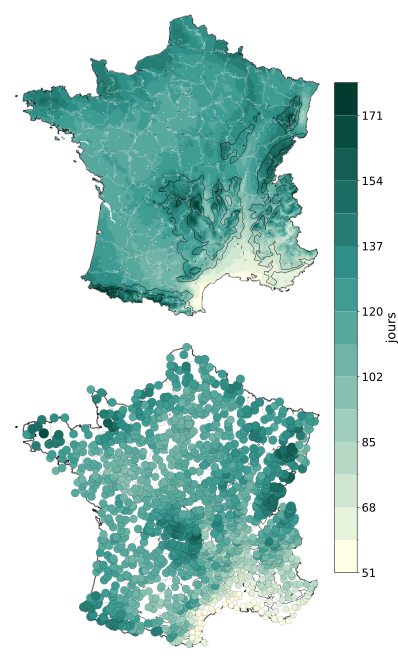
\includegraphics[keepaspectratio]{figures/jour_pluie.pdf}}
&
\pandocbounded{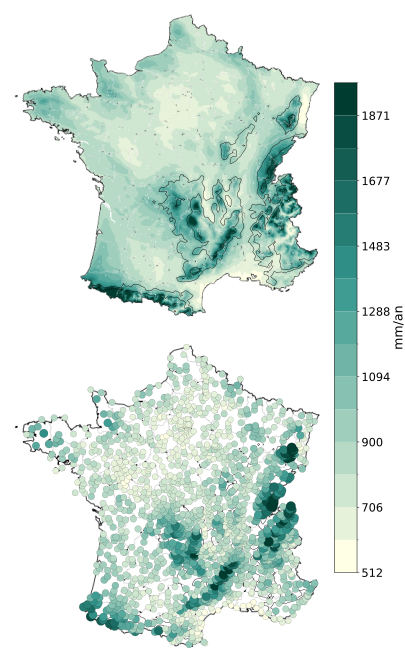
\includegraphics[keepaspectratio]{figures/mean_pluie_jour.pdf}}
&
\pandocbounded{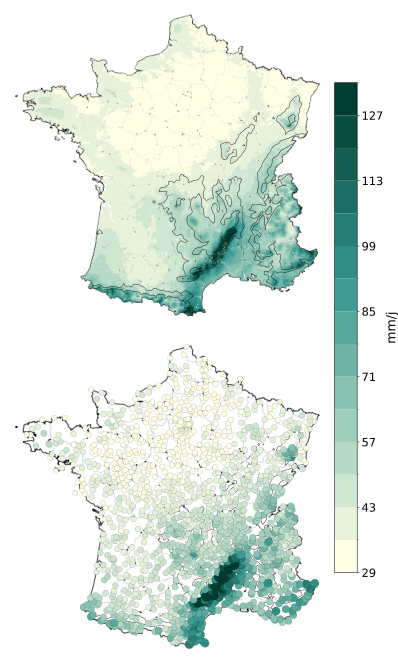
\includegraphics[keepaspectratio]{figures/mean-max_pluie_jour.pdf}} \\
\(r =\) 0.96 (n = 574) & \(r =\) 0.94 (n = 574) & \(r =\) 0.89 (n =
574) \\
\end{longtable}

\begin{center}
Figure 1: Climatologie et corrélation entre le modèle AROME et les stations Météo-France issues de données journalières allant de 1959 à 2022 pour une année hydrologique. Représentation en trait fin des courbes de niveaux 400 et 800m.
\end{center}

\subsubsection{Corrélation entre le modèle AROME et les stations
Météo-France (Figure
2)}\label{corruxe9lation-entre-le-moduxe8le-arome-et-les-stations-muxe9tuxe9o-france-figure-2}

Quelle que soit la climatologie analysée, le modèle \textbf{AROME}
reproduit fidèlement les observations, avec une corrélation minimale de
\textbf{0,70}. Indépendamment de l'échelle temporelle
retenue\,---\,journalière (1959‑2022 ou 1990‑2022) ou horaire
(1990‑2022)\,---\,et de la saison, les champs simulés s'accordent très
bien avec les données mesurées\,: la corrélation varie entre
\textbf{0,92} et \textbf{0,98} pour le nombre de jours de pluie et le
cumul des précipitations.

Cette performance se maintient pour la moyenne des maxima journaliers
(périodes 1959‑2022 et 1990‑2022) sur l'année hydrologique, l'automne,
l'hiver et le printemps, mais elle se dégrade en été, avec une
corrélation de \textbf{0,85}. À l'échelle horaire, la qualité de
l'estimation des maxima se détériore encore\,: la corrélation baisse de
0,4 à 0,8\,point selon la saison pour l'année hydrologique, l'automne et
l'hiver, et chute à environ \textbf{0,70} au printemps et \textbf{0,69}
en été où \(ME =\) -3.753 mm/h (-26.3\%). AROME tend donc à sous-estimer
les précipitations extrêmes estivales, ce qui reste vrai aux autres
saisons.

\includegraphics[width=1\linewidth,height=\textheight,keepaspectratio]{figures/histo_numday_mean_mean-max.png}

\begin{center}
Figure 2: Corrélations des données climatologiques entre le modèle AROME et les stations Météo-France pour chacune des sources de données.
\end{center}

\section{Discussion}\label{discussion}

\subsubsection{Fidélité spatiale de la climatologie
simulée}\label{fiduxe9lituxe9-spatiale-de-la-climatologie-simuluxe9e}

Les résultats confirment qu'AROME reproduit correctement les grands
régimes pluviométriques hexagonaux confirmé par la littérature
\citep{Fumiere2020}, \citep{caillaud2021simulation},
\citep{hess-28-2579-2024}, \citep{LucasPicher2024}. Il y a un excédent
orographique sur les Alpes, les Pyrénées et le Massif central, un
gradient atlantique‑continental marqué à l'ouest\,et un déficit
fréquentiel sur le pourtour méditerranéen. Cette cohérence avec la
réalité mesurée témoigne d'une représentation satisfaisante des forçages
dynamiques (transport d'humidité par les flux d'ouest, soulèvement
orographique, circulation de basse couche en Méditerranée).

\subsubsection{Variabilité saisonnière et représentation des
extrêmes}\label{variabilituxe9-saisonniuxe8re-et-repruxe9sentation-des-extruxeames}

La capacité d'AROME à restituer la fréquence et la quantité de
précipitations se maintient tout au long de l'année, mais la performance
chute pour la moyenne des maxima journaliers en été et davantage à
l'échelle horaire. On retrouve le fait qu'AROME sous-estime des
précipitations d'intensité élévées (\textgreater{} 40 mm/h
\citep{Caillaud2021}) La convection estivale reste partiellement
sous‑résolue malgré la résolution spatiale de 2,5\,km. Dans cette étude,
on a pu montrer (résultats non affichés) que la corrélation augmente
lorsque la fenêtre temporelle s'agrandit à 6 ou 9h. Le modèle pourrait
reproduire la cellule orageuse en\,démarrant trop tard ou trop tôt, en
étalant l'intensité sur plusieurs mailles ou en sous‑estimant les
précipitations maximales. Le pas de 2--3\,km est une étape majeure pour
représenter la convection sans paramétrage, mais il reste trop grossier
pour certaines applications sensibles aux maxima intenses
\citep{Prein2015Review}. Il aurait été intéressant d'introduire les
données COMEPHORE (1\,km, 15\,min) de Météo-France dans cette étude mais
les réanalyses ne débutent qu'en 1997.

\section*{Remerciements}\label{remerciements}
\addcontentsline{toc}{section}{Remerciements}

Je tiens à remercier Juliette Blanchet et Antoine Blanc pour
l'encadrement rigoureux, stimulant et bienveillant tout au long de ce
stage. Leurs conseils avisés, leur disponibilité constante et leurs
nombreuses remarques constructives m'ont permis d'approfondir
considérablement mes compétences scientifiques et méthodologiques. Leur
implication a rendu ce stage particulièrement enrichissant et motivant.
Je leur suis reconnaissant pour leur confiance et leur soutien tout au
long de ce travail.

\section*{References}\label{references}
\addcontentsline{toc}{section}{References}

\renewcommand{\bibsection}{}
\bibliography{bibliography.bib}

\newpage

\section*{Annexes 1 : formules
mathématiques}\label{annexes-1-formules-mathuxe9matiques}
\addcontentsline{toc}{section}{Annexes 1 : formules mathématiques}

\subsection*{A.1.1. Obtention de (1)}\label{a.1.1.-obtention-de-1}
\addcontentsline{toc}{subsection}{A.1.1. Obtention de (1)}

Soit la fonction de vraisemblance
\({\displaystyle {\mathcal {L}}(\theta ;x)} : {\displaystyle \theta \mapsto f(x;\theta )}\).
Alors :
\({\displaystyle \log {\mathcal {L}}(\theta ;x_{1},x_{2},\dots ,x_{n})=\sum _{i=1}^{n}\log {\mathcal {L}}(\theta ;x_{i})}\).

Pour \(1 + \xi \frac{x - \mu}{\sigma} > 0\), avec \(\sigma > 0\) :

\[
\begin{aligned}
\log \mathcal{L}(\theta)
&= \sum_{i=1}^n \left[
  -\log \sigma
  - \frac{1 + \xi}{\xi} \log\left(1 + \xi \frac{x_i - \mu}{\sigma} \right)
  - \left(1 + \xi \frac{x_i - \mu}{\sigma} \right)^{-\frac{1}{\xi}}
\right] \\
\log \mathcal{L}(\theta)
&= -n \log \sigma
- \left(1 + \frac{1}{\xi}\right) \sum_{i=1}^n \log\left(1 + \xi \frac{x_i - \mu}{\sigma} \right)
- \sum_{i=1}^n \left(1 + \xi \frac{x_i - \mu}{\sigma} \right)^{-\frac{1}{\xi}}
\end{aligned}
\]

La log-vraisemblance \(\ell(\theta) = \log \mathcal{L}(\theta)\) s'écrit
alors :

\[
\ell(\theta)=
-\sum_{i=1}^n\Bigl[
\log\sigma
+\Bigl(1+\tfrac1{\xi}\Bigr)\log (1+\xi\;\frac{x_i-\mu}{\sigma})
+(1+\xi\;\frac{x_i-\mu}{\sigma})^{-\frac{1}{\xi}}
\Bigr]
\tag{1}
\]

\subsection*{A.1.2. Obtention des
paramètres}\label{a.1.2.-obtention-des-paramuxe8tres}
\addcontentsline{toc}{subsection}{A.1.2. Obtention des paramètres}

\(\mu_1(z_{T,1})\) et \(\sigma_1(z_{T,1})\)

En développant les paramètres soumis à un effet temporel, on a :

\[
\begin{aligned}
\mu_0 + \mu_1 t &= z_{T,0} + z_{T,1} t - \dfrac{\sigma_0 + \sigma_1 t}{\xi_0} \left[ \left( -\log\left(1 - \frac{1}{T} \right) \right)^{-\xi_0} - 1 \right]\\
\mu_0+\mu_1\,t &= \Bigl[\,z_{T,0}
-\dfrac{\sigma_0}{\xi_0}\Bigl(\bigl[-\log(1-\tfrac1T)\bigr]^{-\xi_0}-1\Bigr)
\Bigr]\;+\;\Bigl[\,z_{T,1}-\dfrac{\sigma_1}{\xi_0}\Bigl(\bigl[-\log(1-\tfrac1T)\bigr]^{-\xi_0}-1\Bigr)\Bigr]\,t\\
\end{aligned}
\]

c'est-à-dire, terme à terme :

\[
\begin{aligned}
\mu_0 &\;=\; z_{T,0}
-\dfrac{\sigma_0}{\xi_0}\Bigl(\bigl[-\log(1-\tfrac1T)\bigr]^{-\xi_0}-1\Bigr),\\[0.8em]
\mu_1 &\;=\; z_{T,1}
-\dfrac{\sigma_1}{\xi_0}\Bigl(\bigl[-\log(1-\tfrac1T)\bigr]^{-\xi_0}-1\Bigr).
\end{aligned}
\]





\end{document}
